\documentclass[14pt]{article}
\usepackage{amsmath}
\usepackage{listings} % For writing code see http://ctan.org/pkg/listings
\usepackage{graphicx}
\usepackage{float}
\usepackage[margin=1.0in]{geometry}
\usepackage{hyperref}

\title{Dynamical model of NGC2419}
\author{Nicolas Garavito-Camargo \& Gurtina Besla}
\begin{document}
\maketitle


In this document different dynamical models of \textbf{NGC2419} are explored
in the presence of the Sagittarius dwarf galaxy (Sgr) and the Large
Magellanic cloud (LMC). The document is structured as follows, in section
\ref{sec:test} the code to compute the orbits is tested with the
public available code \textsc{GalPy}, in section \ref{sec:NGC} the
orbits of NGC2419 are integrating around a spherical MW potential,
in section \ref{sec:NGCSgr} orbits of NGC2419 are integrated in a
spherical MW potential and including the presence of Sgr.
 In the last section \ref{sec:NGCSgrLMC} the orbits of NGC2419 are integrating
with both the presence of Sgr and the LMC.

\section{Testing the code:}\label{sec:test}

A test particle integrated in a NFW profile both with \textsc{Galpy}
and the code developed for this work.

\begin{figure}[H]
\centering
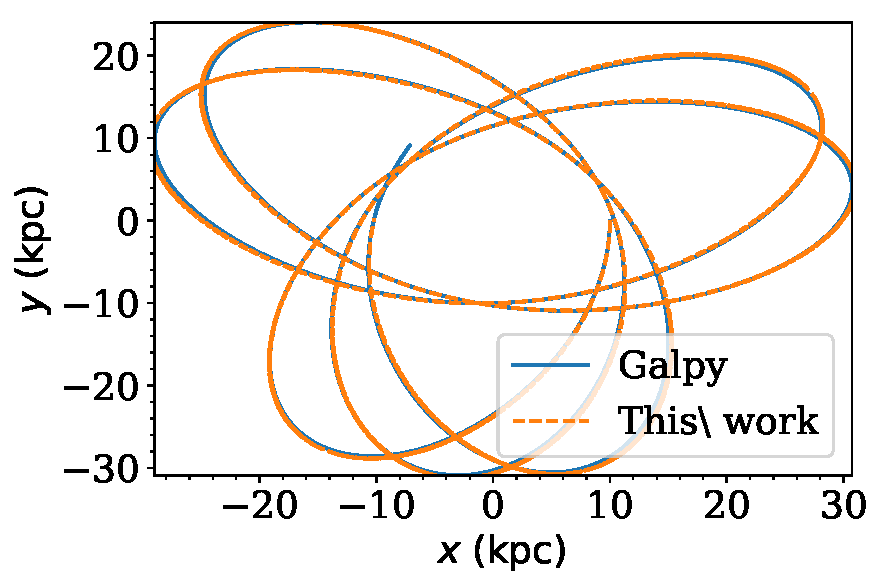
\includegraphics[scale=0.5]{../exploratory_code/galpy_test.pdf}
\end{figure}


\section{The orbit of NGC2419 around the MW}\label{sec:NGC}

Table 1 summarizes the MW model used in the following orbit analyzes.

\begin{table}[H]
\centering
\begin{tabular}{c c c c c}
\hline
\hline
\textbf{Models:} & & & & \\
\hline
\textbf{Model 1:} & & & & \\
Halo: & NFW & $M_{vir} = 1\times 10^{12} M_{\odot}$ & $c=9.86$  \\
Disk: & Miyamoto-Nagai & $M_{d} = 6.5\times10^{10} M_{\odot}$ & $r_L = 3.5 kpc$ & $r_H = 0.53 kpc$ \\
Bulge: & Hernquist & $M_b = 1 \times 10^{10} M_{\odot}$ & $r_s=0.7 kpc$ & \\
%\hline
%\textbf{Model 2:} & & & & \\
%Halo: & NFW & $M_{vir} = 1.5\times 10^{12} M_{\odot}$ & $c=9.56$  \\
%Disk: & Miyamoto-Nagai & $M_{d} = 6.5\times10^{10} M_{\odot}$ & $r_L = 3.5 kpc$ & $r_H = 0.53 kpc$ \\
%Bulge: & Hernquist & $M_b = 1 \times 10^{10} M_{\odot}$ & $r_s=0.7 kpc$ & \\
%\hline
%\textbf{Model 3:} & & & & \\
%Halo: & Triaxial NFW & $M_{vir} = 1.45\times 10^{12} M_{\odot}$ &
%$c=20$  & $q=0.8$, $s=1$. \\
%Disk: & Miyamoto-Nagai & $M_{d} = 4\times10^{10} M_{\odot}$ & $r_L = 3.5 kpc$ & $r_H = 0.53 kpc$ \\
%Bulge: & Hernquist & $M_b = 1 \times 10^{10} M_{\odot}$ & $r_s=0.7 kpc$ & \\
\hline
\hline
\end{tabular}
\caption{Milky Way model parameters}
\end{table}

I'm assuming $q=b/a$, $s=c/a$, $a>b>c$, \textit{In Massari+17 they
mention that $q=0.8$ , but in Hayashi07 they use c/a=0.8 therfore I
think there is a notation problem regardinq the definition of $q$ and
$s$ }\\

Figure \ref{fig:model1MW} shows the projection of the orbits of
NGC2419 for two different initial conditions (blue) using the new
proper motion of Tony and orange using Massari+17 proper motion.
The upper left panel shows the $Y-X$ plane, the upper middle panel
shows the $Z-X$ plane and finally the $Z-Y$ plane is shown in the
upper right panel. The bottom panel shows the galactocentric
distances as a function of time. This two orbits are very different:
The new orbit have a period of $\sim 1.7 Gyrs$ while the old orbit have a
period of $\sim 2.5 gyrs$. The pericenter distances is $\sim 15 kpc$
for the new orbit while for the old orbit is $\sim 65 kpc$.

The angle between the orbital planes is $35.7^{\circ}$, this is best seen in
\href{https://plot.ly/~jngc/3/orbits/?share_key=FcyuVOnd0LYVXaYhGmSuo9}{this}
3D visualization.


\begin{figure}[H]
\centering
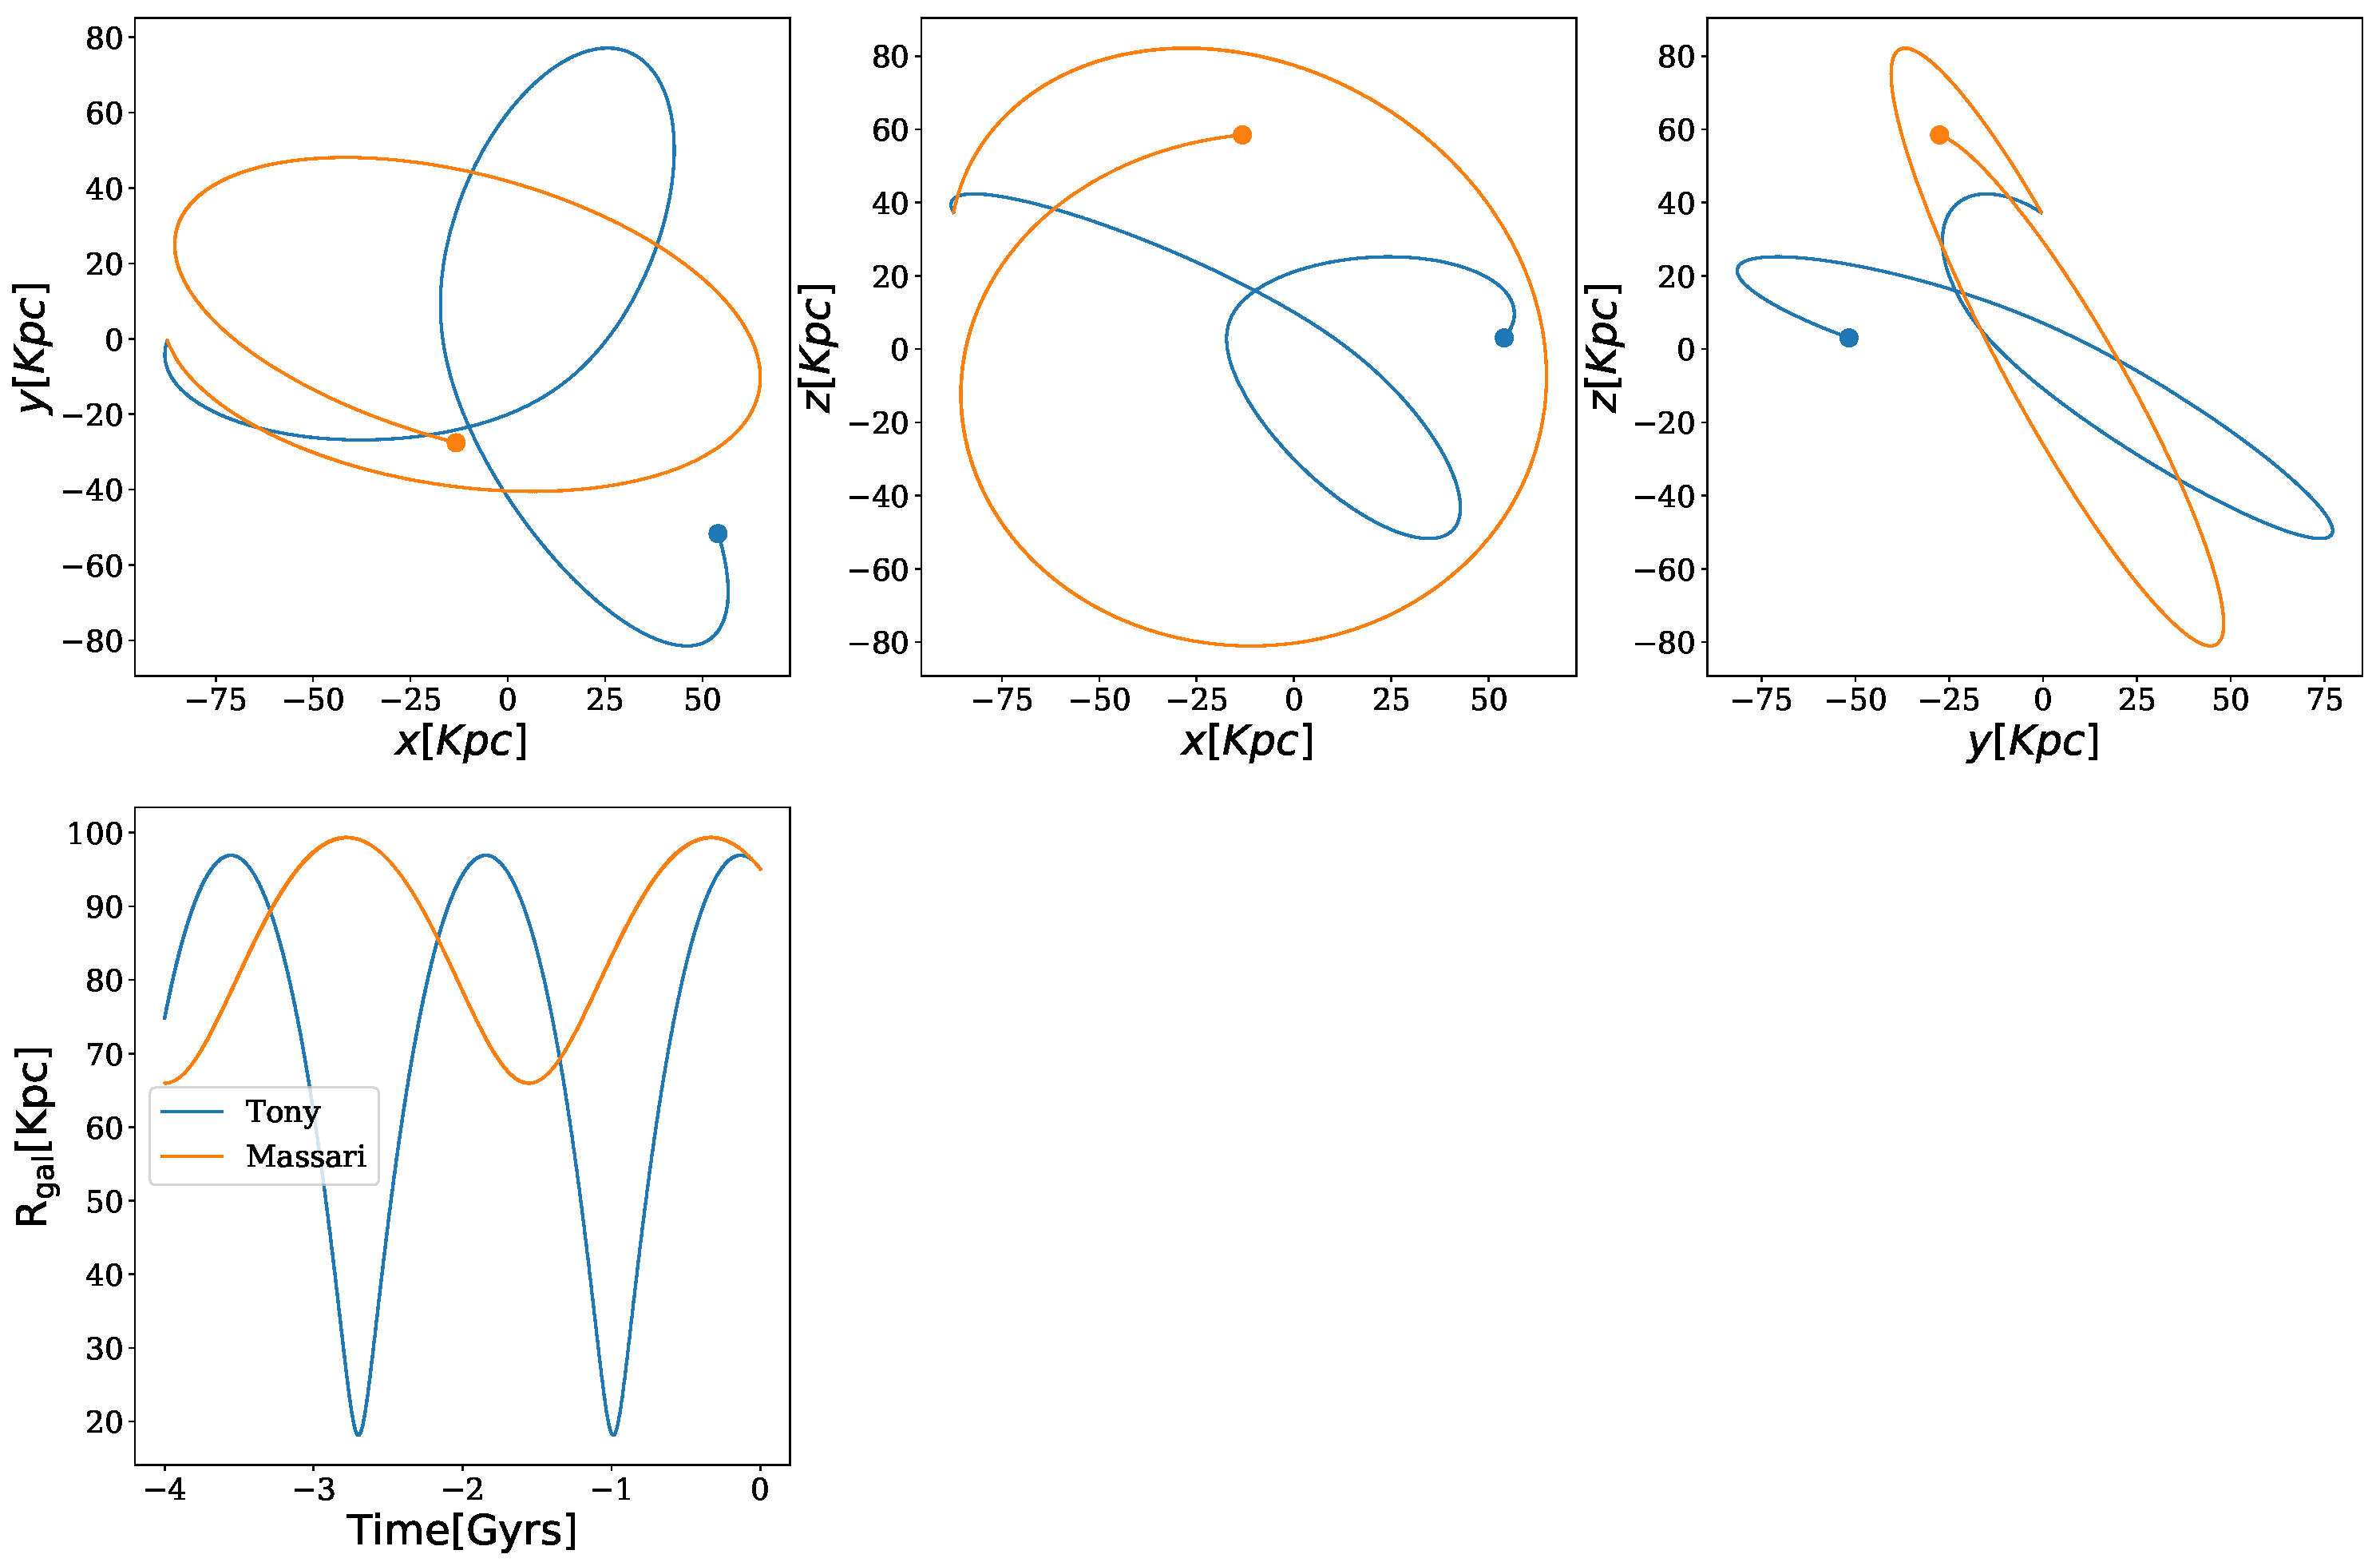
\includegraphics[scale=0.3]{../exploratory_code/NGC2419_sphMW.pdf}
\caption{Orbits of NGC2419 using Model 1, blue line correspond to
the orbit using Tony's proper motions measurements while the orange line correspond to
Massari16 proper motion.\label{fig:model1MW}}
\end{figure}

Figure, shows for a trixial NFW....

\begin{figure}[H]
\centering
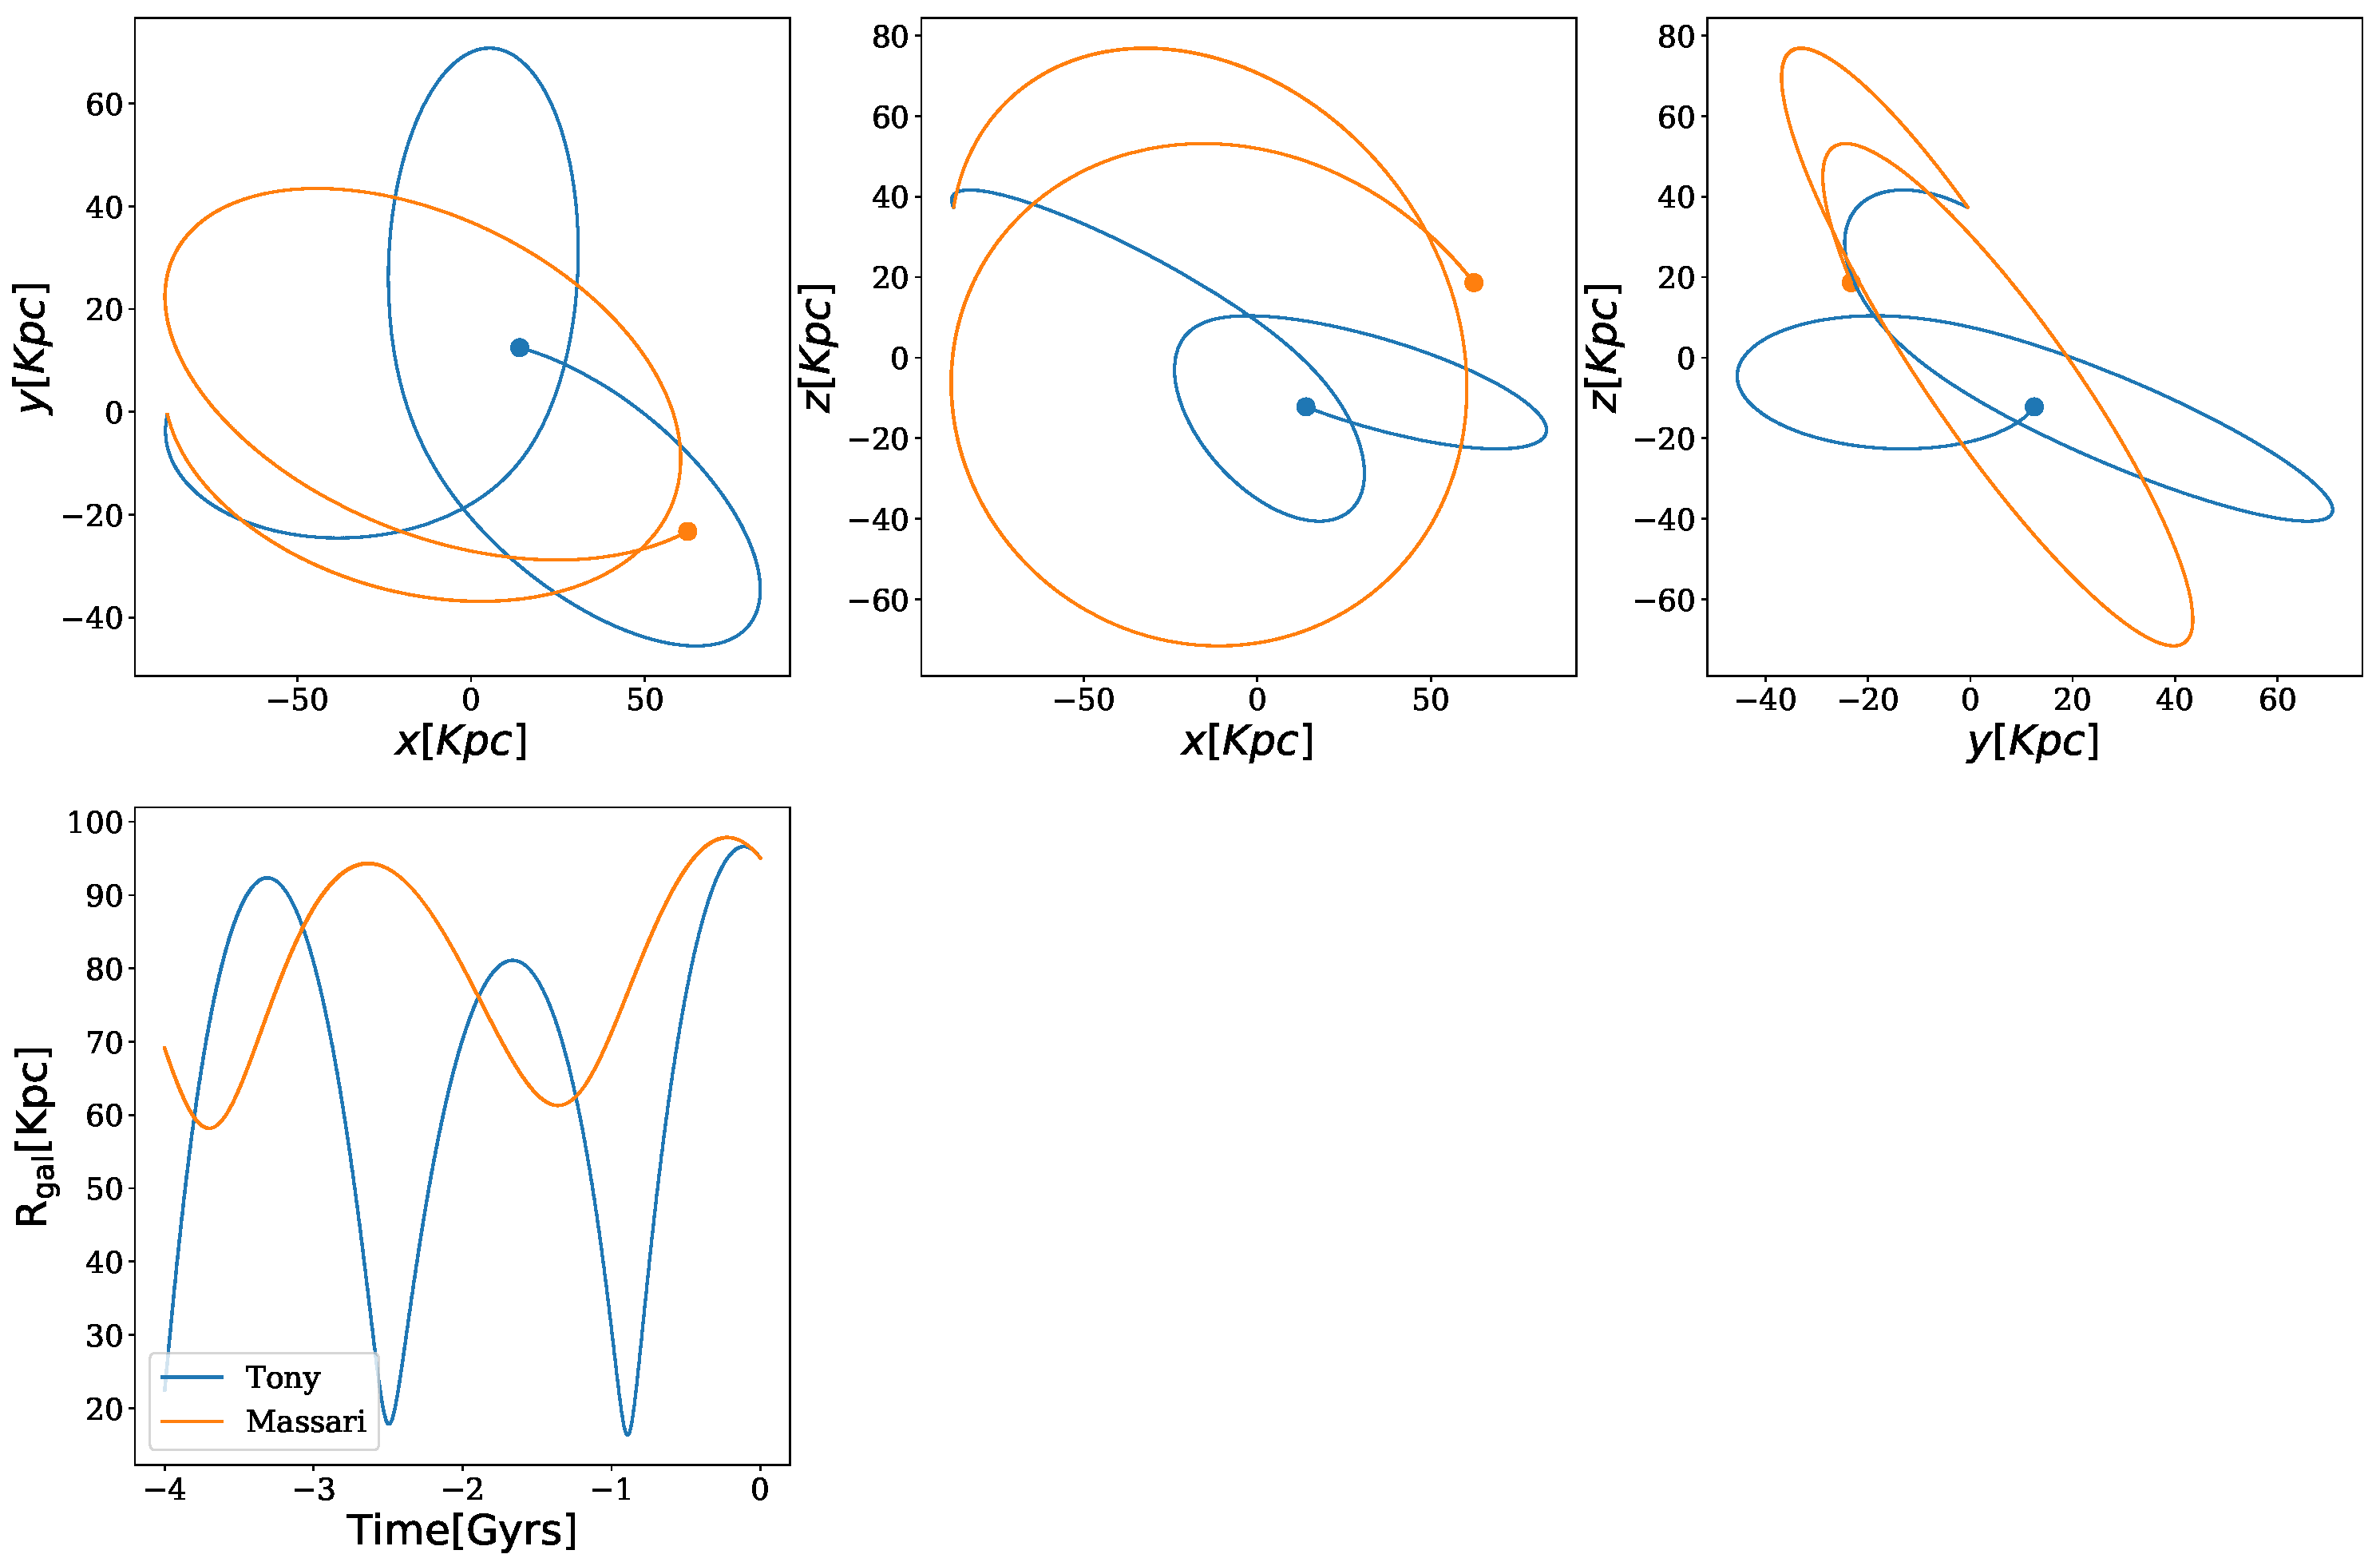
\includegraphics[scale=0.3]{../exploratory_code/NGC2419_Triaxial_MW.pdf}
\caption{Orbits of NGC2419 using model 3. This is the MW model used by
Massari et al 2016.}
\end{figure}



\section{The orbit of NGC2419 around the MW with Sgr}\label{sec:NGCSgr}

In this section we include the effect of the Sagittarius (Sgr) dwarf
galaxy, to this aim we integrate the orbit from the present time. In
this 3-body interaction the MW is free to move due to the
gravitational interaction with Sgr. NGC 2419 feels both the force
from the MW and Sgr. To model the orbit of Sgr we include the dynamic
friction effect by implementing the Chandrasekhar equation, the
Coulomb Logarithm is modified following a similar procedure as the one
in Van Der Marel (XX) in order to account for extended satellites in 
order to reproduce the orbit of Sag from N-body simulations such as 
Diercxx. The model used to represent Sgr is summarized in table
\ref{tab:Sgrmodel}.


\begin{table}[H]
\centering
\begin{tabular}{c c c c c}
\hline
\hline
Halo: & NFW & $M_{vir} = 1\times 10^{10} M_{\odot}$ & $c=8$  \\
\hline
\hline
\end{tabular}
\caption{Sagittarius dwarf model.\label{tab:Sgrmodel}}
\end{table}


Figure \ref{fig:Sgrmodel1} shows the orbit of NGC2419 (Organge) in the
presence of Sgr (Blue), the orbit of NGC2419 using the old proper
motion measurement is shown in green, the blue line shows the tidal
radius of Sgr $r_t = r_{peri} (M_{sat}/(2*M_{MW(r_{peri})}))^{1/3}$.
The angle between the orbits of NGC2419 and Sgr is $55.59$ while the
angle between the plane of the orbit for the old NGC2419  and Sgr is
$24.68$.

\begin{figure}[H]
\centering
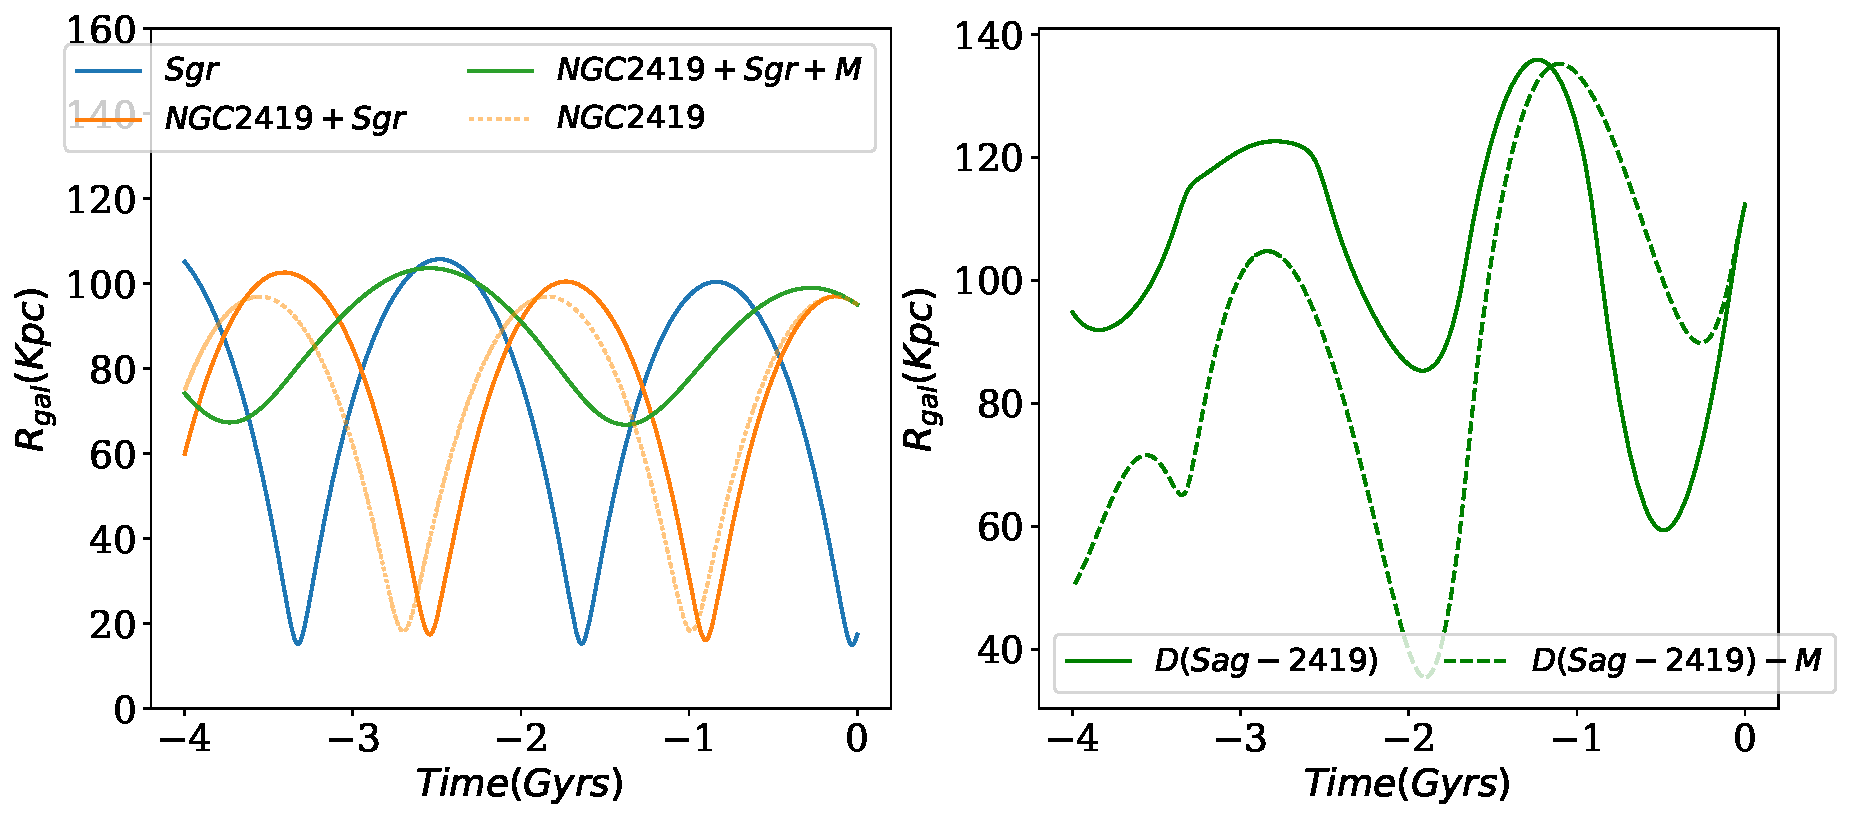
\includegraphics[scale=0.5]{../exploratory_code/NGC2419_sphMWSGR.pdf}
\caption{Right: Orbits of NGC2419 (orange), Sgr (blue), and NGC2419
with Massari+17 proper motion. Left: Distance between NGC2419 and Sgr
as function of time for the new (solid line) and old proper motion
(dashed). \label{fig:Sgrmodel1}}
\end{figure}

A 3D visualization of this plot can be found \href{https://plot.ly/~jngc/22/orbits/}{here}

Finally, sampling the error space of the proper motions of both Sgr
and NGC2419 with $10.000$ initial conditions we explore the properties
of the orbits of NGC2419 for the MW model 1. Figure \ref{fig:all_sgr}
summarize our results, The top left panel shows a histogram of the
time in the orbit of Sgr at which NGC2419 could cross with Sgr or stripped out from Sgr.
The positions on the orbit of Sgr (blue solid line) at which NGC2419 crosses within 
the tidal radius of Sgr at the same time that Sgr is passing trough 
that point in the orbit are shown with orange dots. The top right
panel shows a histogram of polar angles between Sgr and NGC2419.
Bottom left panel shows the histogram of the pericenter distance,
while the apocenter distance is shown in the right bottom panel.

\begin{figure}[H]
\centering
\includegraphics[scale=0.5]{../exploratory_code/all_results_sgr.pdf}
\caption{\label{fig:all_sgr}}
\end{figure}


\section{The orbit of NGC2419 around the MW with Sgr and the
LMC}\label{sec:NGCSgrLMC}

In this section we explore the orbital history of NGC2419 
in the presence of Sgr and the LMC. 
The LMC models are summarized in table \ref{tab:LMCmodels}.


\begin{table}[H]
\centering
\begin{tabular}{c c c c c}
\hline
\hline
Model & Halo potential & $M_{vir} \times 10^{10}M_{\odot}$ & $r_s$ kpc  & \\
LMC1 & Hernquist & $3 $ & $8$  \\
LMC2 & Hernquist & $5 $ & $8$  \\
LMC3 & Hernquist & $8 $ & $8$  \\
LMC4 & Hernquist & $10 $ & $8$  \\
LMC5 & Hernquist & $18 $ & $8$  \\
LMC6 & Hernquist & $25 $ & $8$  \\
\hline
\hline
\end{tabular}
\caption{LMC  models\label{tab:LMCmodels}}
\end{table}


Figure \ref{fig:MWlSgrl} left panel shows the orbits of NGC2419, Sgr and the LMC,
orange, blue and gray respectively with the
LMC (solid lines) and without (dashed lines) for the MW model 1. This figure shows how
the period of Sag decreases and the period of NGC2419 increases thus making
the difference between their periods larger. Right panel shows the
distance between NGC2419 and Sgr at different times, the dashed line
exclude the effect of the LMC.

\begin{figure}[H]
\centering
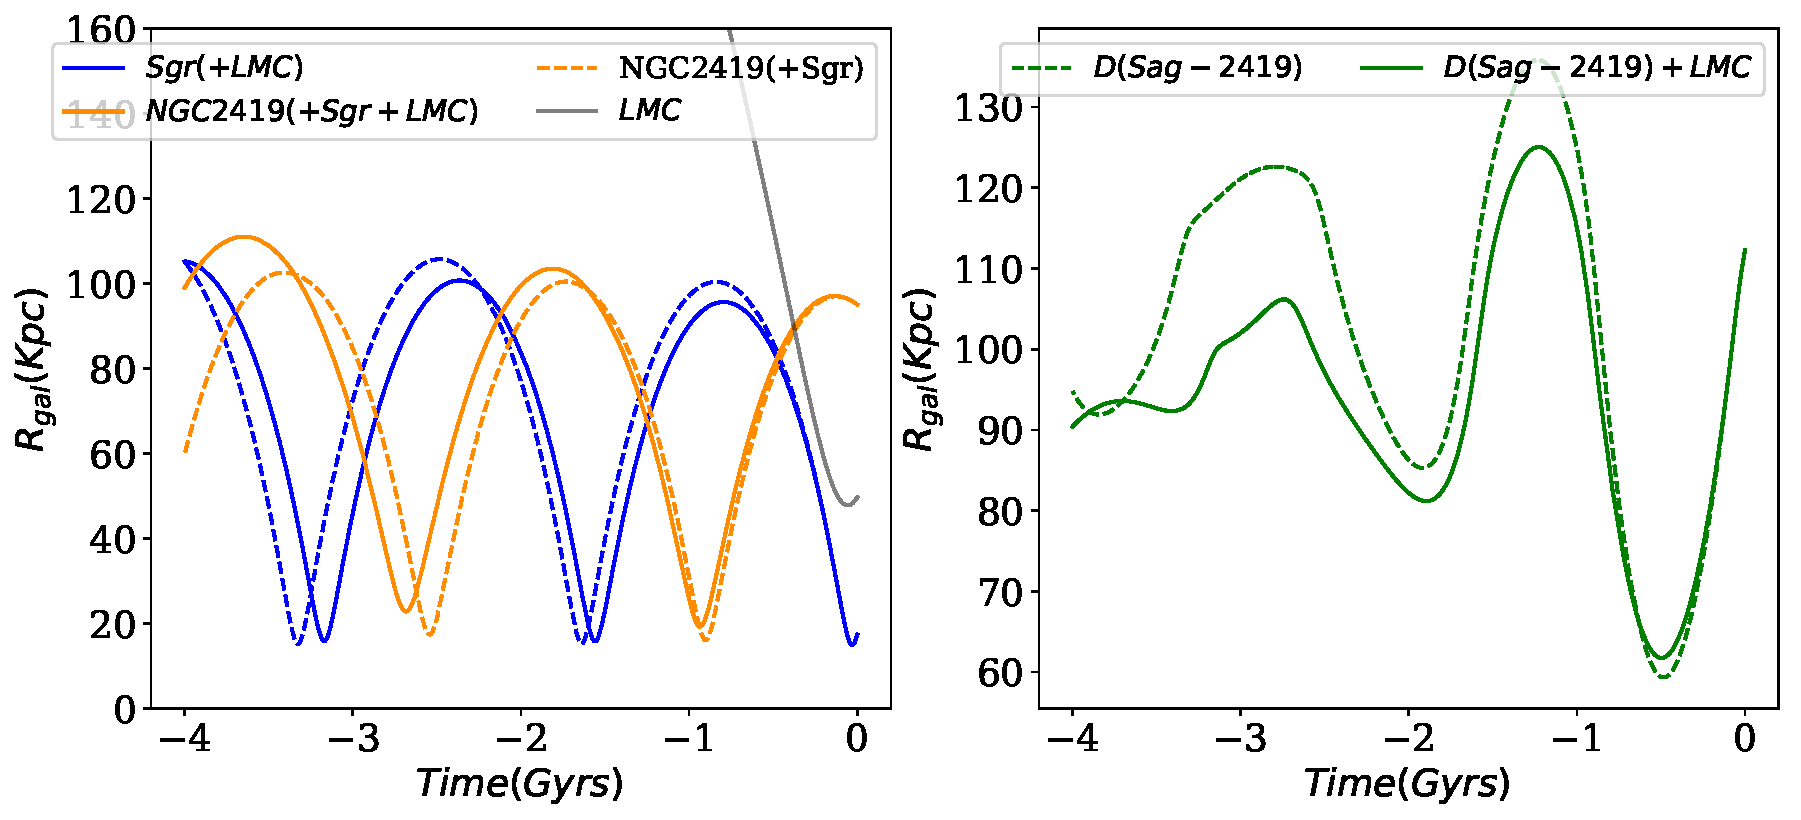
\includegraphics[scale=0.5]{../exploratory_code/NGC2419_sphMWSGRLMC.pdf}
\caption{Model 1 with LMC1 and lightest Sag.\label{fig:MWlSgrl}}
\end{figure}

Figure \ref{fig:MWlSgrh} is the same as figure \ref{fig:MWlSgrl} but
with a heavy Sgr of mass $1\times 10^{11}M_{\odot.}$

\begin{figure}[H]
\centering
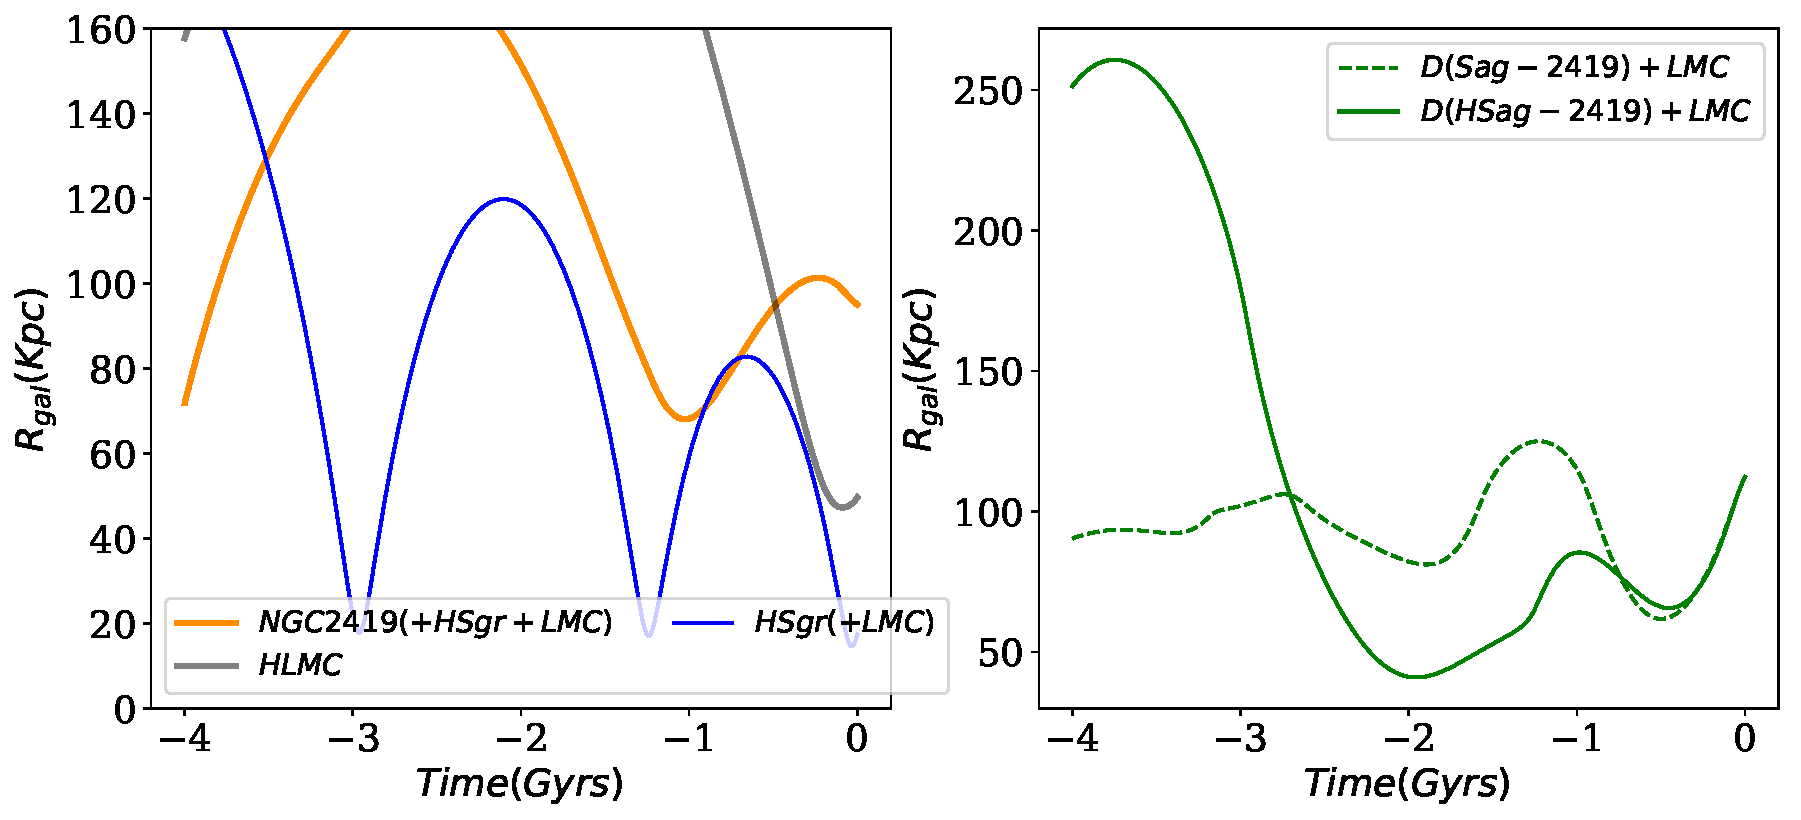
\includegraphics[scale=0.5]{../exploratory_code/NGC2419_sphMWHSGRLMC.pdf}
\caption{for the lightest LMC and Heavy Sag.\label{fig:MWlSgrh}}
\end{figure}

Figure \ref{MWlSgrLMCs} is similar to \ref{fig:MWlSgrl} but for the
six models of the LMC, the thiner the lines the more massive the LMC.


\begin{figure}[H]
\centering
\begin{minipage}{0.49\linewidth}
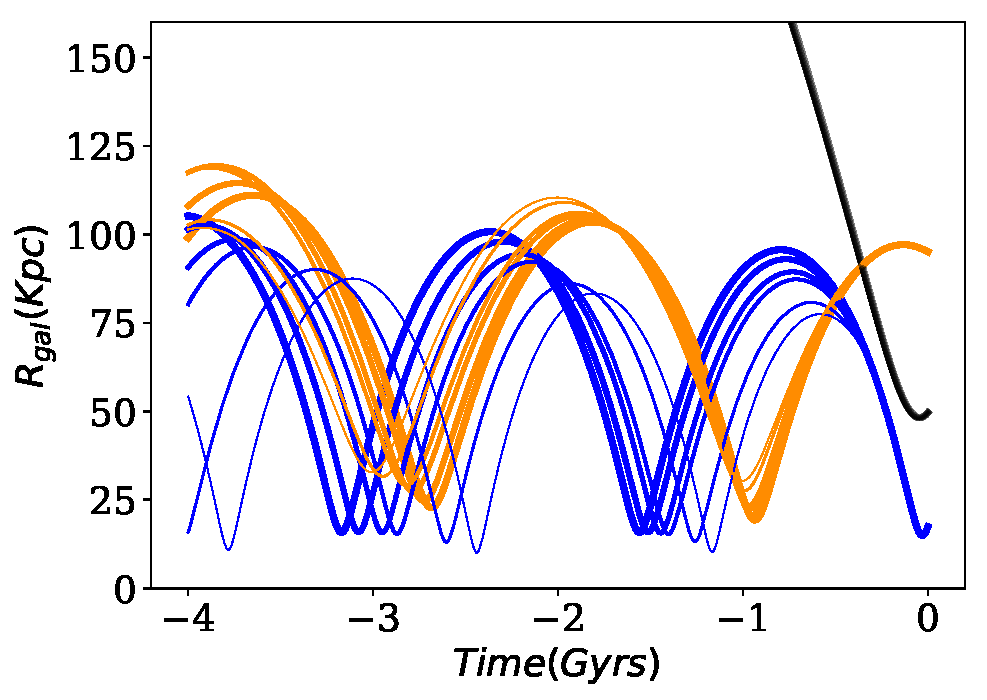
\includegraphics[scale=0.5]{../exploratory_code/gal_orbits_all_LMCs.pdf}
\end{minipage}
\begin{minipage}{0.45\linewidth}
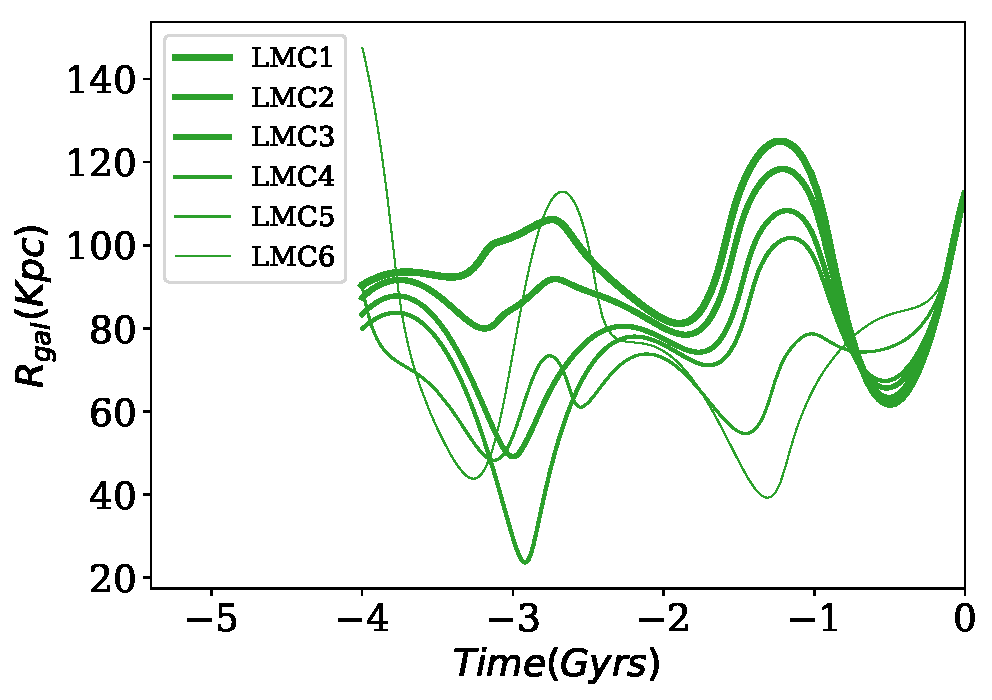
\includegraphics[scale=0.5]{../exploratory_code/d_rel_all_LMCs.pdf}
\end{minipage}
\caption{Left: Galactocentric distances for NGC2419, Sgr and the LMC (Blue,
orange and black respectively. Right: Relative distances between
NGC2419 and Sgr.)\label{fig:MWlSgrLMCs}}
\end{figure}


\begin{figure}[H]
\centering
\includegraphics[scale=0.5]{../exploratory_code/all_results_sgrlmc.pdf}
\caption{Results using 10000 orbits integrated from sampling the
error space for NGC2419 and Sgr. Top left panel shows the minimum
distance that NGC2419 gets to Sgr at a given time, the blue horizontal
line represents the Sgr tidal radius. Top right panel shows an
histogram of the orbital poles angle of NGC2419 and Sgr. Bottom left
panel shows a histogram of the pericenter distance of NGC2419 and
the bottom wight panel shows a histogram of the apocenter
distance.}
\end{figure}

\end{document}

